\documentclass[11pt,a4paper]{article}

\usepackage[a4paper,margin=0.75in]{geometry}
\usepackage{booktabs}
\usepackage{array}
\usepackage{tabularx}
\usepackage{amsmath,amssymb,amsfonts}
\usepackage[table]{xcolor}
\usepackage{ragged2e}
\usepackage{tikz}
\usetikzlibrary{shapes.geometric,arrows.meta,positioning,calc,fit}
\usepackage{hyperref}
\usepackage{listings}
\usepackage{microtype}
\usepackage{float}
\usepackage{enumitem}

% ── Modern Color Palette Definition ──────────────────────────────────────────
\definecolor{primaryblue}{RGB}{37,99,235}
\definecolor{accentblue}{RGB}{29,78,216}
\definecolor{darkgray}{RGB}{31,41,55}
\definecolor{lightbg}{RGB}{249,250,251}
\definecolor{bordergray}{RGB}{229,231,235}
\definecolor{codegreen}{RGB}{22,163,74}
\definecolor{dangerred}{RGB}{220,38,38}
\definecolor{purpleaccent}{RGB}{124,58,237}
\definecolor{headergray}{RGB}{243,244,246}
\definecolor{amberorange}{RGB}{217,119,6}

\hypersetup{
    colorlinks=true,
    linkcolor=primaryblue,
    citecolor=primaryblue,
    urlcolor=primaryblue
}

\renewcommand{\familydefault}{\sfdefault}
\setlength{\parindent}{0pt}
\setlength{\parskip}{5pt}
\renewcommand{\arraystretch}{1.25}

\title{\textbf{\LARGE Comprehensive Technical Report: System Architecture, Core Modules, and Repository Inventory}\\[0.4em]
\large Real-Time Eye-Tracking, Virtual Keyboard AAC Platform \& Experimental Text-Entry Framework}
\author{\textbf{Eye-Tracking Research \& Accessibility Engineering Group}}
\date{\today}

\begin{document}

\maketitle

\begin{abstract}
This report delivers an exhaustive, in-depth architectural and functional summary of the codebase present in this repository. The platform represents an end-to-end, webcam-based assistive technology system engineered for hands-free computer interaction, Augmentative and Alternative Communication (AAC), and Human-Computer Interaction (HCI) text-entry experimentation. Operating entirely on consumer-grade RGB cameras without specialized infrared hardware, the system integrates deep-learning facial landmarking (MediaPipe Face Landmarker), geometric iris localization, real-time Eye Aspect Ratio (EAR) blink detection, 6-DOF head-pose estimation, exponential moving average (EMA) jitter suppression, and dwell-time interaction engines. Additionally, the repository includes multi-layout on-screen keyboards (QWERTY, Alphabetical, Frequency-Clustered), an emergency phrase dispatch utility with multi-channel routing (Twilio SMS and Webhooks), high-resolution gaze heatmap rendering (2D Gaussian KDE), and automated experimental logging and LaTeX reporting. In accordance with project instructions, all analytical post-processing and quiz-specific modules have been strictly omitted from this inventory.
\end{abstract}

\tableofcontents
\newpage

% =============================================================================
\section{Executive Summary \& Repository Overview}
% =============================================================================

The repository provides a complete, production-ready assistive computing environment designed to empower motor-impaired individuals, locked-in patients, and HCI researchers. The platform enables full hands-free text entry, emergency signaling, and standardized psychomotor typing experiments through webcam ocular tracking. 

The software framework combines low-level computer vision, real-time signal filtering, multi-threaded operating system hooks (Windows Win32 API), graphical interfaces (Tkinter and embedded Microsoft Edge WebView2), and automated artifact generators.

\begin{figure}[H]
\centering
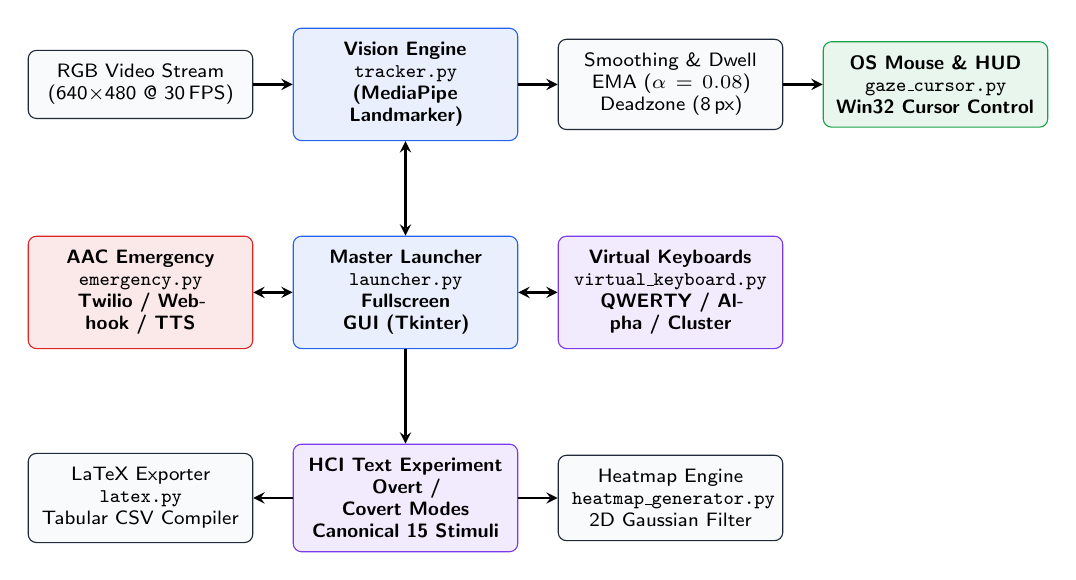
\begin{tikzpicture}[
    node distance=0.7cm and 0.5cm,
    >=stealth,
    every node/.style={transform shape, font=\scriptsize},
    box/.style={rectangle, draw=darkgray, fill=lightbg, rounded corners=3pt, align=center, inner sep=5pt, text width=2.5cm},
    primarybox/.style={rectangle, draw=primaryblue, fill=primaryblue!10, rounded corners=3pt, align=center, inner sep=5pt, text width=2.5cm, font=\scriptsize\bfseries},
    greenbox/.style={rectangle, draw=codegreen, fill=codegreen!10, rounded corners=3pt, align=center, inner sep=5pt, text width=2.5cm, font=\scriptsize\bfseries},
    purplebox/.style={rectangle, draw=purpleaccent, fill=purpleaccent!10, rounded corners=3pt, align=center, inner sep=5pt, text width=2.5cm, font=\scriptsize\bfseries},
    redbox/.style={rectangle, draw=dangerred, fill=dangerred!10, rounded corners=3pt, align=center, inner sep=5pt, text width=2.5cm, font=\scriptsize\bfseries}
]

    \node (cam) [box] {RGB Video Stream\\(640$\times$480 @ 30\,FPS)};
    \node (tracker) [primarybox, right=of cam] {Vision Engine\\\texttt{tracker.py}\\(MediaPipe Landmarker)};
    \node (filter) [box, right=of tracker] {Smoothing \& Dwell\\EMA ($\alpha=0.08$)\\Deadzone (8\,px)};
    \node (cursor) [greenbox, right=of filter] {OS Mouse \& HUD\\\texttt{gaze\_cursor.py}\\Win32 Cursor Control};

    \node (launcher) [primarybox, below=1.2cm of tracker] {Master Launcher\\\texttt{launcher.py}\\Fullscreen GUI (Tkinter)};
    \node (vkb) [purplebox, right=of launcher] {Virtual Keyboards\\\texttt{virtual\_keyboard.py}\\QWERTY / Alpha / Cluster};
    \node (emergency) [redbox, left=of launcher] {AAC Emergency\\\texttt{emergency.py}\\Twilio / Webhook / TTS};

    \node (exp) [purplebox, below=1.2cm of launcher] {HCI Text Experiment\\Overt / Covert Modes\\Canonical 15 Stimuli};
    \node (heatmap) [box, right=of exp] {Heatmap Engine\\\texttt{heatmap\_generator.py}\\2D Gaussian Filter};
    \node (latex) [box, left=of exp] {LaTeX Exporter\\\texttt{latex.py}\\Tabular CSV Compiler};

    \draw[->, thick] (cam) -- (tracker);
    \draw[->, thick] (tracker) -- (filter);
    \draw[->, thick] (filter) -- (cursor);
    \draw[<->, thick] (launcher) -- (tracker);
    \draw[<->, thick] (launcher) -- (vkb);
    \draw[<->, thick] (launcher) -- (emergency);
    \draw[->, thick] (launcher) -- (exp);
    \draw[->, thick] (exp) -- (heatmap);
    \draw[->, thick] (exp) -- (latex);

\end{tikzpicture}
\caption{System macro-architecture and component interaction diagram.}
\label{fig:macro_arch}
\end{figure}

% =============================================================================
\section{Comprehensive File \& Directory Inventory}
% =============================================================================

The repository comprises executable Python scripts, neural model binary assets, configuration schemas, experiment datasets, and artifact generation utilities. Table~\ref{tab:file_inventory} catalogs the primary components present in the workspace.

\begin{table}[H]
\centering
\caption{Complete Inventory of Project Modules, Scripts, and Assets (Excluding Analysis/Quiz).}
\label{tab:file_inventory}
\small
\begin{tabularx}{\textwidth}{p{0.22\textwidth} p{0.14\textwidth} p{0.15\textwidth} X}
\toprule
\textbf{File / Directory} & \textbf{Type} & \textbf{Primary Technology} & \textbf{Functional Purpose \& Description} \\
\midrule
\texttt{launcher.py} & Python Script & Tkinter, WebView2 & Master application portal; controls fullscreen navigation, tracker subprocess lifecycle, embedded browser chat, and the full experimental testing harness. \\
\texttt{tracker.py} & Python Script & OpenCV, MediaPipe & Core computer vision pipeline; computes facial landmarks, iris gaze tracking, EAR blink classification, head pose, dwell clicks, and HUD overlays. \\
\texttt{emergency.py} & Python Script & Tkinter, Twilio, SAPI & Augmentative communication suite; offers emergency phrase boards, text-to-speech audio, and multi-channel remote signaling (Twilio SMS/Webhooks). \\
\texttt{virtual\_keyboard.py} & Python Script & OpenCV, PyAutoGUI & High-contrast on-screen keyboard rendering engine with multiple layout schemes, dwell selection bars, and direct TextPad linkage. \\
\texttt{text\_pad.py} & Python Script & OpenCV & Floating text composition canvas featuring dwell-driven action buttons (Save, Clear, Layout Switch) and gaze point recording. \\
\texttt{gaze\_cursor.py} & Python Script & OpenCV & Visual gaze HUD cursor renderer with outer pulsing rings, crosshairs, sci-fi brackets, and temporal smoothing. \\
\texttt{heatmap\_generator.py} & Python Script & Matplotlib, SciPy & High-resolution gaze attention density mapping engine using 2D Gaussian spatial convolutions and peak hotspot extraction. \\
\texttt{latex.py} & Python Script & Pandas, LaTeX & Automated compilation tool converting experiment trial CSV data into publication-grade landscape LaTeX tables. \\
\texttt{keyboardaccuracy.py} & Python Script & Tkinter & Dedicated keyboard evaluation interface with integrated Notepad and accuracy logging. \\
\texttt{generate\_flowchart.py}& Python Script & PIL (Pillow) & Programmatic visual tree diagram generator rendering repository architectures into high-resolution PNGs. \\
\texttt{face\_landmarker.task}& Binary Asset & TensorFlow Lite & Pre-trained MediaPipe 3D face mesh model containing 478 canonical facial and iris landmark geometries. \\
\texttt{emergency\_config.json}& JSON Config & JSON & Persistent configuration storing emergency phone numbers, dispatch channels, Twilio credentials, and phrase presets. \\
\texttt{calibration\_profiles.json} & JSON Database & JSON & Persistent database of facial geometry embeddings and customized gaze/EAR thresholds for returning users. \\
\texttt{usage\_stats.json} & JSON Storage & JSON & Session duration and cumulative system usage tracking log. \\
\texttt{Real\_test/} & Directory & CSV, TXT & Data repository storing structured experimental trial outputs from live participant sessions. \\
\texttt{latex/} & Directory & TeX, PDF & Storage directory for generated LaTeX experiment tables and comprehensive architecture reports. \\
\texttt{heatmaps/} & Directory & PNG Images & Storage repository for generated 2D spatial gaze fixation heatmaps. \\
\bottomrule
\end{tabularx}
\end{table}

% =============================================================================
\section{Master Launcher \& Central Hub (\texttt{launcher.py})}
% =============================================================================

The master launcher serves as the system orchestrator, process supervisor, and user gateway. Built with Tkinter and styled with a modern design system, it operates in fullscreen kiosk mode with automated crash recovery.

\subsection{Architectural \& Threading Model}
To support modern web technologies alongside low-latency computer vision, the launcher employs a dual-threading model:
\begin{itemize}
    \item \textbf{Single-Threaded Apartment (STA) Main Thread}: Uses PythonNet (\texttt{clr}) to initialize the Tkinter event loop in an STA thread, satisfying Microsoft Edge WebView2 runtime COM requirements.
    \item \textbf{Decoupled Subprocess Supervisor}: Launches \texttt{tracker.py} in an independent Python process via \texttt{subprocess.Popen}, preventing GUI frame drops during intensive video processing.
    \item \textbf{Flag-Based Inter-Process Communication}: Coordinates tracker execution and pause states using filesystem flags (\texttt{calib\_done.flag} and \texttt{tracker\_paused.flag}).
\end{itemize}

\subsection{Core Modules Accessible from the Launcher}
\begin{enumerate}
    \item \textbf{Eye Tracker Card}: Triggers returning-user verification, calibration, and launches the live tracking background process.
    \item \textbf{Emergency Communication Card}: Launches the hands-free AAC emergency signaling and phrase interface (\texttt{EmergencyWindow}).
    \item \textbf{Notepad with On-Screen Keyboard}: Provides a full-featured text editor with zoomable typography, word-wrap toggles, and an embedded virtual keyboard.
    \item \textbf{Text-Entry Experiment}: Executes standardized cognitive-motor typing trials with automated metric computation and CSV logging.
    \item \textbf{Embedded WebView2 Browser}: Features a dedicated web navigation window (\texttt{BrowserWindow}) with navigation bars, search queries, and secure web rendering.
\end{enumerate}

% =============================================================================
\section{Real-Time Eye \& Attention Tracking Engine (\texttt{tracker.py})}
% =============================================================================

The tracking engine \texttt{tracker.py} is the core computational module. It processes live webcam frames at 30\,FPS to deliver sub-pixel gaze estimation, blink classification, and head-pose orientation.

\subsection{Landmark Geometry \& Iris Extraction}
The system utilizes the MediaPipe Face Landmarker Tasks API, extracting 478 3D landmarks ($x, y, z$). Key facial regions are indexed as follows:
\begin{itemize}
    \item \textbf{Left Iris}: Landmarks [474, 475, 476, 477]
    \item \textbf{Right Iris}: Landmarks [469, 470, 471, 472]
    \item \textbf{Left Eye Eyelid Contour}: Landmarks [33, 160, 158, 133, 153, 144]
    \item \textbf{Right Eye Eyelid Contour}: Landmarks [362, 385, 387, 263, 373, 380]
\end{itemize}
Iris centers are computed by taking the minimum enclosing circle or midpoint of opposite iris points, delivering normalized coordinates $I_x, I_y \in [0, 1]$.

\subsection{Mathematical Formulations}

\subsubsection{1. Eye Aspect Ratio (EAR) for Blink Discrimination}
Eye openness is determined by calculating the ratio between the vertical distances of opposite eyelid landmarks and the horizontal width:
\begin{equation}
\text{EAR} = \frac{\|P_{160} - P_{144}\|_2 + \|P_{158} - P_{153}\|_2}{2 \|P_{33} - P_{133}\|_2 + \epsilon}
\end{equation}
where $\|A - B\|_2 = \sqrt{(x_A - x_B)^2 + (y_A - y_B)^2}$ is the 2D Euclidean distance and $\epsilon = 10^{-6}$ prevents zero-division. 

A deliberate left blink triggers a mouse click under the following conditions:
\begin{equation}
\text{Click}_{\text{left}} = 
\begin{cases}
1, & \text{if } \text{EAR}_L < \theta_{\text{EAR}} \text{ for } N_f \in [4, 20] \text{ frames, } (t - t_{\text{last}}) > T_{\text{cool}}, \text{ and } \text{Head} = \text{FORWARD} \\
0, & \text{otherwise}
\end{cases}
\end{equation}
where $\theta_{\text{EAR}} = 0.23$, $N_f = 4$ frames ($\approx 133\,\text{ms}$) eliminates micro-blinks, $N_f \le 20$ filters out prolonged closures (drowsiness), and $T_{\text{cool}} = 0.90\,\text{s}$ prevents accidental re-triggering.

\subsubsection{2. 6-DOF Head-Pose Estimation}
The rigid $4 \times 4$ transformation matrix $M$ provided by MediaPipe is sliced to obtain the $3 \times 3$ rotation matrix $R \in SO(3)$. Euler angles are derived as:
\begin{align}
\text{Yaw}   &= \arctan2\left(R_{1,0}, R_{0,0}\right) \times \frac{180^\circ}{\pi} \\
\text{Pitch} &= \arctan2\left(-R_{2,0}, \sqrt{R_{2,1}^2 + R_{2,2}^2}\right) \times \frac{180^\circ}{\pi}
\end{align}
Postural stability is validated against operational limits: $|\text{Yaw}| \le 25^\circ$ and $|\text{Pitch}| \le 20^\circ$. If exceeded, the system flags the user as distracted and locks click interactions.

\subsubsection{3. Gaze-to-Screen Mapping \& Spatial Calibration}
Normalized iris positions $g_x, g_y$ are mapped to physical screen coordinates $(s_x, s_y)$ through a calibrated 4-parameter bounding box $[x_{\min}, x_{\max}, y_{\min}, y_{\max}]$:
\begin{equation}
s_x = \text{clip}\left(\frac{g_x - x_{\min}}{x_{\max} - x_{\min}}, 0, 1\right) \times W_{\text{screen}}, \quad
s_y = \text{clip}\left(\frac{g_y - y_{\min}}{y_{\max} - y_{\min}}, 0, 1\right) \times H_{\text{screen}}
\end{equation}

\subsubsection{4. Temporal Exponential Moving Average (EMA) \& Deadzone Gaze Smoothing}
To suppress involuntary ocular tremors (4--7\,px physiological drift) while maintaining responsive cursor movement, a non-linear gated filter is applied:
\begin{align}
d &= \sqrt{(s_{x, t} - \hat{s}_{x, t-1})^2 + (s_{y, t} - \hat{s}_{y, t-1})^2} \\
\hat{s}_t &= 
\begin{cases}
\hat{s}_{t-1}, & \text{if } d \le \delta_{\text{deadzone}} \\
\alpha s_t + (1 - \alpha) \hat{s}_{t-1}, & \text{if } d > \delta_{\text{deadzone}}
\end{cases}
\end{align}
where $\delta_{\text{deadzone}} = 8\,\text{px}$, $\alpha = 0.08$ (providing 92\% inertial smoothing), and maximum displacement per frame is bounded by $\Delta_{\max} = 40\,\text{px}$.

\subsubsection{5. Anti-Midas Touch Dwell-to-Click Engine}
Hands-free clicking without eyelid strain is achieved through spatial fixation monitoring:
\begin{equation}
P_{\text{dwell}}(t) = \min\left(1.0, \frac{t - t_{\text{anchor}}}{T_{\text{dwell}}}\right)
\end{equation}
where $T_{\text{dwell}} = 1.50\,\text{s}$ is the hold duration, $\mathcal{R}_{\text{dwell}} = 35\,\text{px}$ is the allowable jitter radius around the anchor, and $T_{\text{cooldown}} = 1.80\,\text{s}$ enforces post-selection safety lockout.

\subsection{Multi-Phase Calibration Pipeline}
The calibration process guarantees high-fidelity tracking across diverse lighting conditions and subjects:
\begin{itemize}
    \item \textbf{Phase 0 (Automated Returning User Recognition)}: Computes a 120-dimensional normalized geometric face embedding vector across 16 key facial landmarks. If the Mean Squared Error (MSE) compared against any entry in \texttt{calibration\_profiles.json} satisfies $\text{MSE} < 0.0015$, previous calibration thresholds ($\text{EAR}_L, \text{EAR}_R, \text{gaze\_calib}$) are loaded instantly, bypassing manual calibration.
    \item \textbf{Phase 0.5 (Face Position \& Height Alignment)}: Displays an interactive semi-transparent ellipse guide. Evaluates facial height ($0.24 \le h_{\text{face}} \le 0.65$) and vertical center ($0.38 \le y_{\text{center}} \le 0.58$), giving real-time feedback (``SIT HIGHER'', ``MOVE CLOSER'').
    \item \textbf{Phase 1 (Baseline EAR Acquisition)}: Samples eyelid distances over 3 seconds to establish individual blink baselines ($\mu - 1.5\sigma - 0.02$).
    \item \textbf{Phase 2 (Active 4-Corner Fixation Mapping)}: Sequentially presents targets at display corners. Demands 1.2 seconds of steady fixation ($\sigma_x, \sigma_y < 0.007$) before recording 10th and 90th percentile bounding boundaries.
\end{itemize}

% =============================================================================
\section{AAC Emergency System (\texttt{emergency.py})}
% =============================================================================

Designed for urgent patient communication, \texttt{emergency.py} delivers a high-contrast Augmentative and Alternative Communication (AAC) interface operating independently or via gaze clicks.

\subsection{Functional Capabilities}
\begin{itemize}
    \item \textbf{Color-Coded Tile Layout}:
    \begin{itemize}
        \item \emph{Green Tiles (Medical \& Care Needs)}: Urgent phrases such as \emph{``I need immediate help!''}, \emph{``I am in severe pain''}, \emph{``Please bring me water''}, and \emph{``Please call emergency services!''}.
        \item \emph{Orange Tiles (Rapid Dialogue Responses)}: Fast affirmation/negation keys: \emph{``Yes''}, \emph{``No''}, \emph{``Maybe''}, \emph{``Please''}, \emph{``Thank you''}.
    \end{itemize}
    \item \textbf{Multi-Channel Signal Dispatch}:
    \begin{itemize}
        \item \emph{Simulation Mode}: Internal verification channel with audit trail logging.
        \item \emph{Twilio REST API}: Authenticates via Account SID and Auth Token to dispatch live SMS alerts to configured caregiver phone numbers.
        \item \emph{HTTP Webhook}: Posts structured JSON payloads to hospital or emergency endpoints.
    \end{itemize}
    \item \textbf{Multi-Modal Alarms \& TTS}:
    \begin{itemize}
        \item Fires background audio alarm bursts (2500\,Hz beeps via \texttt{winsound}).
        \item Synthesizes vocal speech via \texttt{pyttsx3} with fallback to Windows SAPI PowerShell commands.
    \end{itemize}
    \item \textbf{Audit Logging \& Storage}: Appends every dispatched alert, timestamp, recipient number, and transmission channel to \texttt{emergency\_sent\_log.txt}.
\end{itemize}

% =============================================================================
\section{Hands-Free Virtual Keyboards \& Text Pad (\texttt{virtual\_keyboard.py}, \texttt{text\_pad.py})}
% =============================================================================

The repository provides modular, on-screen text input systems optimized for gaze-driven selection.

\subsection{Keyboard Layout Topologies}
The keyboard engine supports three selectable layouts:
\begin{enumerate}
    \item \textbf{QWERTY (Standard)}: Familiar universal arrangement for literate users.
    \item \textbf{Alphabetical (A--Z)}: Systematic 3-row layout facilitating linear visual search for novice AAC users.
    \item \textbf{Frequency-Clustered}: Positions high-frequency English characters (\texttt{E, T, A, O, I, N, S, H}) at central visual fixations, reducing total saccadic travel distance.
\end{enumerate}

\subsection{Keyboard Architecture \& Control Features}
\begin{itemize}
    \item \textbf{Integrated 3$\times$4 Numpad}: Right-aligned numeric cluster (\texttt{1--9, 0, ., ?}) aligned with alphabet rows.
    \item \textbf{Dedicated Editing Row}: Horizontal bottom row containing navigation and edit keys: \texttt{|◄} (Start of Line), \texttt{◄} (Left), \texttt{⌫} (Backspace), \texttt{Space}, \texttt{Delete} (Clear All), \texttt{►} (Right), and \texttt{►|} (End of Line).
    \item \textbf{Visual Dwell Charging}: Displays expanding colored rings and inverted highlights during dwell progress ($T_{\text{dwell}} = 1.20\,\text{s}$).
\end{itemize}

\subsection{Floating TextPad Module}
\texttt{text\_pad.py} provides an independent $700 \times 500$\,px text composition canvas. It features:
\begin{itemize}
    \item Gaze-accessible action buttons: \texttt{ALPHA KB}, \texttt{QWERTY KB}, and \texttt{CLUSTER KB}.
    \item Automatic text buffering with space management.
    \item Live norm-coordinate gaze accumulator (\texttt{record\_gaze}) that feeds the heatmap rendering pipeline upon saving.
\end{itemize}

% =============================================================================
\section{Text-Entry Experimentation Framework (\texttt{launcher.py}, \texttt{Real\_test/})}
% =============================================================================

A key research capability in this repository is the psychomotor text-entry experiment engine hosted inside \texttt{launcher.py}. It enables controlled, scientific benchmarking of gaze typing speed and accuracy.

\subsection{Experimental Testing Paradigms}
\begin{enumerate}
    \item \textbf{Overt Method (Memory-Loaded Typing)}:
    \begin{itemize}
        \item A target stimulus is presented during a 15-second memorization window.
        \item The stimulus disappears completely when the typing keyboard appears.
        \item Evaluates working memory retention, mental transcription speed, and recall degradation under gaze tracking.
    \end{itemize}
    \item \textbf{Covert Method (Concurrent Visual Typing)}:
    \begin{itemize}
        \item The target prompt remains permanently visible above the input area throughout the trial.
        \item Isolates pure visual search, motor targeting, and eye-hand coordination latency.
    \end{itemize}
\end{enumerate}

\subsection{Stimulus Organization \& Standardized Corpus}
Sessions consist of 15 standardized trials drawn from a canonical corpus:
\begin{itemize}
    \item \textbf{10 Canonical Words}: \texttt{help}, \texttt{food}, \texttt{sleep}, \texttt{Doctor}, \texttt{Medicine}, \texttt{Water}, \texttt{Pain}, \texttt{Uncomfortable}, \texttt{family}, \texttt{Friends}.
    \item \textbf{5 Standard Pangrams / Phrases}:
    \begin{enumerate}
        \item \emph{``The quick brown fox jumps over the lazy dog.''}
        \item \emph{``I agree with you''}
        \item \emph{``a little encouragement is needed''}
        \item \emph{``I would like to go home''}
        \item \emph{``the computer is running slowly''}
    \end{enumerate}
\end{itemize}
Stimuli are delivered either in a \textbf{Fixed Interleaved Sequence} (blocks of 2 words followed by 1 phrase, repeated 5 times) or a \textbf{Random Sequence} (shuffled pool of all 15 items).

\subsection{Experimental Rigor \& Protocol Controls}
\begin{itemize}
    \item \textbf{Center-Cursor Warping (\texttt{\_center\_cursor})}: Calls Win32 \texttt{SetCursorPos} to reposition the mouse pointer to the exact screen center ($(W/2, H/2)$) before each trial and after every break, standardizing visual search latency across trials.
    \item \textbf{30-Second Inter-Trial Rest Break}: Displays an animated countdown bar between trials, plays auditory audio beeps, speaks voice reminders via TTS, and creates \texttt{tracker\_paused.flag} to suspend vision loop processing and prevent eye fatigue.
    \item \textbf{Granular Keystroke Timestamping}: Captures the relative timestamp ($\pm 1$\,ms) of every character, space, and backspace entered, serializing the keystroke sequence into JSON format within the trial log.
\end{itemize}

% =============================================================================
\section{Heatmap Generation Engine (\texttt{heatmap_generator.py})}
% =============================================================================

\texttt{heatmap\_generator.py} visualizes spatial eye attention across sessions by transforming raw coordinate logs into full-resolution ($1920 \times 1080$) PNG heatmaps.

\subsection{Algorithmic Formulation}
Given a series of normalized gaze fixations $\{(x_i, y_i)\}_{i=1}^N \in [0, 1]^2$, the process executes as follows:
\begin{enumerate}
    \item \textbf{Grid Binning}: Maps points to an internal discrete 2D matrix $\mathcal{D} \in \mathbb{R}^{H_g \times W_g}$ where $W_g = 400$ and $H_g = \lfloor 400 / (W_{\text{screen}} / H_{\text{screen}}) \rfloor$.
    \item \textbf{2D Gaussian Kernel Filtering}: Convolves the discrete accumulation grid with a Gaussian blur kernel:
    \begin{equation}
    \mathcal{G}(x, y) = \frac{1}{2\pi \sigma^2} \exp\left(-\frac{x^2 + y^2}{2\sigma^2}\right), \quad \sigma = 0.03 \times W_g
    \end{equation}
    \item \textbf{Intensity Normalization}: Normalizes peak density: $\tilde{\mathcal{D}} = \mathcal{D} / \max(\mathcal{D})$.
    \item \textbf{Custom Colormap Mapping}: Applies a 5-stop RGBA transfer function transitioning from fully transparent $\rightarrow$ translucent cyan $\rightarrow$ teal-green $\rightarrow$ amber $\rightarrow$ opaque red.
    \item \textbf{Hotspot Centroid Extraction}: Computes and highlights the top-5 gaze density centroids with indexed callout circles (\#1 through \#5).
\end{enumerate}

% =============================================================================
\section{Automated Reporting \& Flowchart Generators (\texttt{latex.py}, \texttt{generate_flowchart.py})}
% =============================================================================

The repository contains automated tools for converting experimental session data into formal scientific documentation.

\subsection{Automated LaTeX Exporter (\texttt{latex.py})}
\texttt{latex.py} automatically compiles experiment CSV logs into publication-ready LaTeX tables. Its capabilities include:
\begin{itemize}
    \item Parsing CSV metadata: participant identifiers, sequence modes, and layout choices.
    \item Generating landscape tabular sections comparing trial stimulus strings, typed responses, character counts, and durations.
    \item Parsing serialized keystroke timestamp arrays into multi-line tabular cells (formatted as \texttt{char:sec}).
    \item Auto-escaping special TeX symbols (\%, \$, \_, \&, \#).
\end{itemize}

\subsection{Visual File Hierarchy Generator (\texttt{generate\_flowchart.py})}
\texttt{generate\_flowchart.py} uses Pillow to construct a $2400 \times 2800$\,px high-resolution flowchart depicting the project structure (\texttt{file\_structure\_flowchart.png}). It renders color-coded folder icons, file type badges, connecting trunks, and branch indicators.

% =============================================================================
\section{Data Formats, Schemas \& System Protocols}
% =============================================================================

The system maintains clean data structures across all storage media. Table~\ref{tab:schemas} outlines the schema definitions implemented across the repository.

\begin{table}[H]
\centering
\caption{System Data Schemas and Storage Formats.}
\label{tab:schemas}
\small
\begin{tabularx}{\textwidth}{p{0.25\textwidth} p{0.25\textwidth} X}
\toprule
\textbf{File / Storage Format} & \textbf{Key Fields / Columns} & \textbf{Data Types \& Descriptions} \\
\midrule
\textbf{Experiment CSV Logs} \newline (\texttt{Real\_test/real\_test\_csv/*.csv}) & \texttt{participant\_name}, \texttt{trial\_number}, \texttt{method}, \texttt{sequence\_mode}, \texttt{keyboard\_layout}, \texttt{stimulus}, \texttt{typed\_response}, \texttt{is\_correct}, \texttt{typing\_duration\_sec}, \texttt{spacebar\_count}, \texttt{backspace\_count}, \texttt{char\_count}, \texttt{letter\_timestamps} & Strings, integers, floats, booleans, and JSON-encoded lists of keystroke timestamp pairs \texttt{[[char, time], ...]}. Records complete psychomotor trial performance. \\
\midrule
\textbf{Continuous Gaze Log} \newline (\texttt{gaze\_log.csv}) & \texttt{timestamp}, \texttt{gaze\_x}, \texttt{gaze\_y}, \texttt{blink}, \texttt{gaze\_dir}, \texttt{head\_status}, \texttt{ear\_left}, \texttt{ear\_right} & Float timestamps, normalized coordinates ($[0, 1]$), binary blink flags, direction strings (CENTER/LEFT/RIGHT), head posture strings, and instantaneous EAR values. \\
\midrule
\textbf{Calibration Database} \newline (\texttt{calibration\_profiles.json}) & \texttt{embedding}, \texttt{EAR\_TH\_L}, \texttt{EAR\_TH\_R}, \texttt{gaze\_calib}, \texttt{timestamp} & 120-element float distance vector, float EAR thresholds, 4-element gaze calibration bounds $[x_{\min}, x_{\max}, y_{\min}, y_{\max}]$, and timestamp string. \\
\midrule
\textbf{Emergency Config} \newline (\texttt{emergency\_config.json}) & \texttt{emergency\_contact}, \texttt{dispatch\_channel}, \texttt{twilio\_*}, \texttt{webhook\_url}, \texttt{phrases} & Configuration dictionary containing contact numbers, dispatch modes, API keys, and category-tagged phrase lists. \\
\midrule
\textbf{State Synchronization Flags} \newline (\texttt{*.flag}) & \texttt{calib\_done.flag}, \texttt{tracker\_paused.flag} & Filesystem synchronization signals coordinating GUI restoration and tracker video pause states. \\
\bottomrule
\end{tabularx}
\end{table}

% =============================================================================
\section{Conclusion}
% =============================================================================

The repository presents an integrated, highly functional assistive technology and research ecosystem. By combining consumer webcam computer vision (MediaPipe), mathematically rigorous signal filtering (EAR, Euler head pose, EMA deadzone smoothing), and accessible GUI architectures (AAC phrase boards, multi-layout keyboards, and standardized HCI text experiments), the codebase provides a self-contained platform for hands-free computing. Automated heatmap synthesis, file hierarchy generation, and LaTeX compilation ensure that experimental findings and operational states can be evaluated and reported with scientific rigor.

\end{document}
